\subsubsection{Backend Technologies}
\paragraph{Go}
At the start of the project, a portion of the team deliberated about which
technologies to choose for the backend. Options using JavaScript such as NodeJS
or Deno with accompanying frameworks like ExpressJS or NestJS were considered,
as was Rust and its Rocket framework. They would have been excellent choices as
they are well established in the industry and tried-and-tested.

The majority of the team has development experience with JavaScript, so going
with that would have made a lot of sense. However, it was planned from the very
beginning to deploy this application on a server hosted by one of the team
members. Therefore, the usage of computing and memory resources was very
important to them, as they did not want to strain their Kubernetes cluster more
than necessary. Since NodeJS runs on the JavaScript runtime V8, which also
powers Google Chrome, our experience indicated that it would be quite resource
intensive to run.

Due to this, the team shifted towards using compiled rather than interpreted
languages, as these are generally more resource efficient. Since small
executables and low memory usage was desired, languages and frameworks that run
on virtual machines such as Java with Spring or C\# with .Net were not deemed to
be viable options. As a result, only Rust and Go were seriously considered at
this point.

Rust offers a small package size, strong memory safety, an excellent
ecosystem and build-tools. The team member that would focus on backend
development had recent experience in writing Rust code. However, Rust
development can be very tricky and time consuming. Additionally, in our
experience Rust has above average compilation times. In a project with a fixed
deadline and the expectation of rapid development, choosing Rust would have been
detrimental. The team recognised that choosing Rust would come with many
drawbacks while offering only few benefits.

This left choosing Go as the logical conclusion. A large drawback that the team
identified with Go was the missing experience in the team. Two team members had
used Go before, but they last used it a few years back. However, since Go syntax
and the languages concepts hadn't changed much since then, it was deemed
possible to quickly get up to speed, much more quickly than Rust would have
allowed. The final decision fell on using Go, as it offered small binaries,
great memory efficiency, a solid ecosystem of libraries and build-tools and a
feature-rich, built-in library for creating REST-APIs. Go also removes a lot of
the pitfalls that Rust suffers from: it has a simple and approachable syntax and
a very low-friction, high-speed development experience. This was also the
deciding factor, since it was made clear to the team that getting an MVP up and
running as quickly as possible was imperative for the project.

\paragraph{PostgreSQL}
The plan for the MVP of Magpie set the simple goal of delivering useful data to
users. To achieve this, the data needs to be stored in a way in which it can be
efficiently accessed during operation. Since the goal of the project was to
provide a tool to professionals, data integrity at every level was an important
consideration. Additional requirements for the data storage solution were good
support for geospatial data, quick retrieval of a large number of points and
ease-of-use.

There is a plethora of database solutions available today. The team considered
the most common types: document databases like MongoDB and multi-model databases
like PostgreSQL (sometimes called RDBMS).

While document databases like MongoDB have their place in the current
development landscape, it soon became clear that SQL-based, multi-model RDBMSs
would be best suited for the job. They offer tried-and-tested performance and
reliability and they are well equipped to guarantee data integrity. But the
deciding reason was the pre-existing experience the lead developer for the
backend had with these types of databases.

After some deliberation, PostgreSQL was chosen as the database solution for this
project. It was combined with the PostGIS extension to add support for
geospatial data and queries. The decision was not cut and dried as most
established multi-model databases (like Oracle DB or MySQL) offer the
functionality that the requirements were asking for. However, the Kubernetes
cluster this project was going to be deployed on already had a fully configured
PostgreSQL server running on it. Making use of pre-existing infrastructure is
the obvious choice in an agile project that had the prime goal of hitting the
ground running.

\paragraph{sqlc}
In modern software development, there are two common ways for an application to
interact with a database via SQL. There is the old school way of writing raw SQL
queries, put them into prepared statements and execute them against the
database. This gives the developer very granular control over the way their
queries are structured and how they run them. But this method requires a
significant amount of work in designing and implementing a translation layer
between the database and the application. Data that the application wants to
send to the database needs to be prepared into a format the database queries
expect. Data that the application wants to retrieve from the database needs to
be parsed back into the data model that's used by the application.

To make interfacing with databases easier, so called ORMs (Object Relational
Models) were developed. These are libraries that the application developer can
include. Database queries are not done in SQL, but in the same programming
language the application is written in. The ORM provides database interface
functions that take in the data in the format the application uses. To actually
perform any queries or make any changes to the database, the ORM runs its own
SQL queries against the database via a compatible driver internally. ORMs
abstract away the direct communication with the database and provide a simpler
wrapper in the programming language that is used anyway. This can make it easier
and quicker to develop an application that makes use of a database, but it takes
away some of the agency that the developer has.


The team wasn't really happy with either of these solutions, so an alternative
called sqlc was chosen. This tool combines the freedom that using SQL gives
developers with the productivity increase that ORMs offer. sqlc flips the
typical ORM workflow on its head. This means, the developer writes standard SQL
queries and schemas which are then passed to the CLI of sqlc. In accordance with
a configuration file provided by the developer, sqlc then automatically
generates type-safe bindings for the queries that were defined in the SQL files
(\cite{sqlc_introduction}).

This approach gives the developer more control about the queries that are
executed. At the same time, it eliminates the need to write boilerplate wrapper
code for accessing the database, just like an ORM would eliminate the need to
write SQL queries. The tool treats SQL, which is a structured and typed
language, as a source of truth. It also enables developers to reuse their
queries across systems as sqlc offers code generation for multiple programming
languages like Go, Python or Typescript and databases like PostgreSQL, MySQL or
SQLite (\cite{sqlc_documentation_language_support}).

The tool respects best practices to prevent SQL injection attacks. It generates
code that only utilises constant strings and parametrised queries
(\cite{sqlc_injection}). Using a tool like this, the team was quickly able to
connect the backend server to the database. Eliminating the need to update the
Go code manually each time the database schema or queries changed was vital for
the backend keeping pace with the other developers.

\begin{listing}[htbp]
  \centering{}
  \begin{minipage}{0.75\textwidth}
  \begin{minted}{yaml}
      version: "2"
      sql:
      - schema: "sql/migrations"
        queries: "sql/queries_private.sql"
        engine: "postgresql"
        gen:
          go:
            package: "db"
            sql_package: "pgx/v5"
            out: "internal/db/private"
            build_tags: "private"
            emit_json_tags: true
            overrides:
              - db_type: "geometry"
                go_type:
                  import: "github.com/twpayne/go-geom"
                  pointer: true
                  type: "Point"
      - schema: "sql/migrations"
        queries: "sql/queries_public.sql"
        engine: "postgresql"
        gen:
          go:
            package: "db"
            sql_package: "pgx/v5"
            out: "internal/db/public"
            build_tags: "public"
            emit_json_tags: true
            overrides:
              - db_type: "geometry"
                go_type:
                  import: "github.com/twpayne/go-geom"
                  pointer: true
                  type: "Point"
  \end{minted}
  \end{minipage}
  \caption{An example of a sqlc configuration file with two targets with separate query inputs}
  \label{listing:sqlc_config_file}
\end{listing}

\begin{listing}[htbp]
  \centering{}
  \begin{minipage}{\textwidth}
  \begin{minted}{sql}
    -- name: GetPointsInRadius :many
    SELECT Id, LongLat::geometry, Type from points
    WHERE ST_DWithin(
      LongLat::geography,
      ST_SetSRID(ST_MakePoint(@longitude::float, @latitude::float), 4326)::geography,
      @radius::float
    ) AND (
      @types::point_type[] IS NULL OR Type = ANY(@types::point_type[])
    );
  \end{minted}
  \end{minipage}
  \caption{An example of a SQL query with annotations used by sqlc}
  \label{listing:sqlc_query_input}
\end{listing}

\begin{listing}[htbp]
  \centering{}
  \begin{minipage}{0.85\textwidth}
  \begin{minted}{go}
    const getPointsInRadius = `-- name: GetPointsInRadius :many
    SELECT Id, LongLat::geometry, Type from points
    WHERE ST_DWithin(
      LongLat::geography,
      ST_SetSRID(ST_MakePoint($1::float, $2::float), 4326)::geography,
      $3::float
    ) AND (
      $4::point_type[] IS NULL OR Type = ANY($4::point_type[])
    )
    `

    type GetPointsInRadiusParams struct {
      Longitude float64     `json:"longitude"`
      Latitude  float64     `json:"latitude"`
      Radius    float64     `json:"radius"`
      Types     []PointType `json:"types"`
    }

    type GetPointsInRadiusRow struct {
      ID      int64          `json:"id"`
      Longlat *go_geom.Point `json:"longlat"`
      Type    PointType      `json:"type"`
    }

    func (q *Queries) GetPointsInRadius(
        ctx context.Context, arg GetPointsInRadiusParams
      ) ([]GetPointsInRadiusRow, error) {
      rows, err := q.db.Query(ctx, getPointsInRadius,
        arg.Longitude,
        arg.Latitude,
        arg.Radius,
        arg.Types,
      )
      if err != nil {
        return nil, err
      }
      defer rows.Close()
      var items []GetPointsInRadiusRow
      for rows.Next() {
        var i GetPointsInRadiusRow
        if err := rows.Scan(&i.ID, &i.Longlat, &i.Type); err != nil {
          return nil, err
        }
        items = append(items, i)
      }
      if err := rows.Err(); err != nil {
        return nil, err
      }
      return items, nil
    }
  \end{minted}
  \end{minipage}
  \caption{An example of a Go binding generated by sqlc from the SQL query in
  Listing \ref{listing:sqlc_query_input}}
  \label{listing:sqlc_generated_bindings}
\end{listing}


\paragraph{golang-migrate}

The complete database development workflow for the backend server is visualised
in Figure \ref{fig:database_workflow_diagram}.

\begin{figure}[htbp]
  \centering{}
  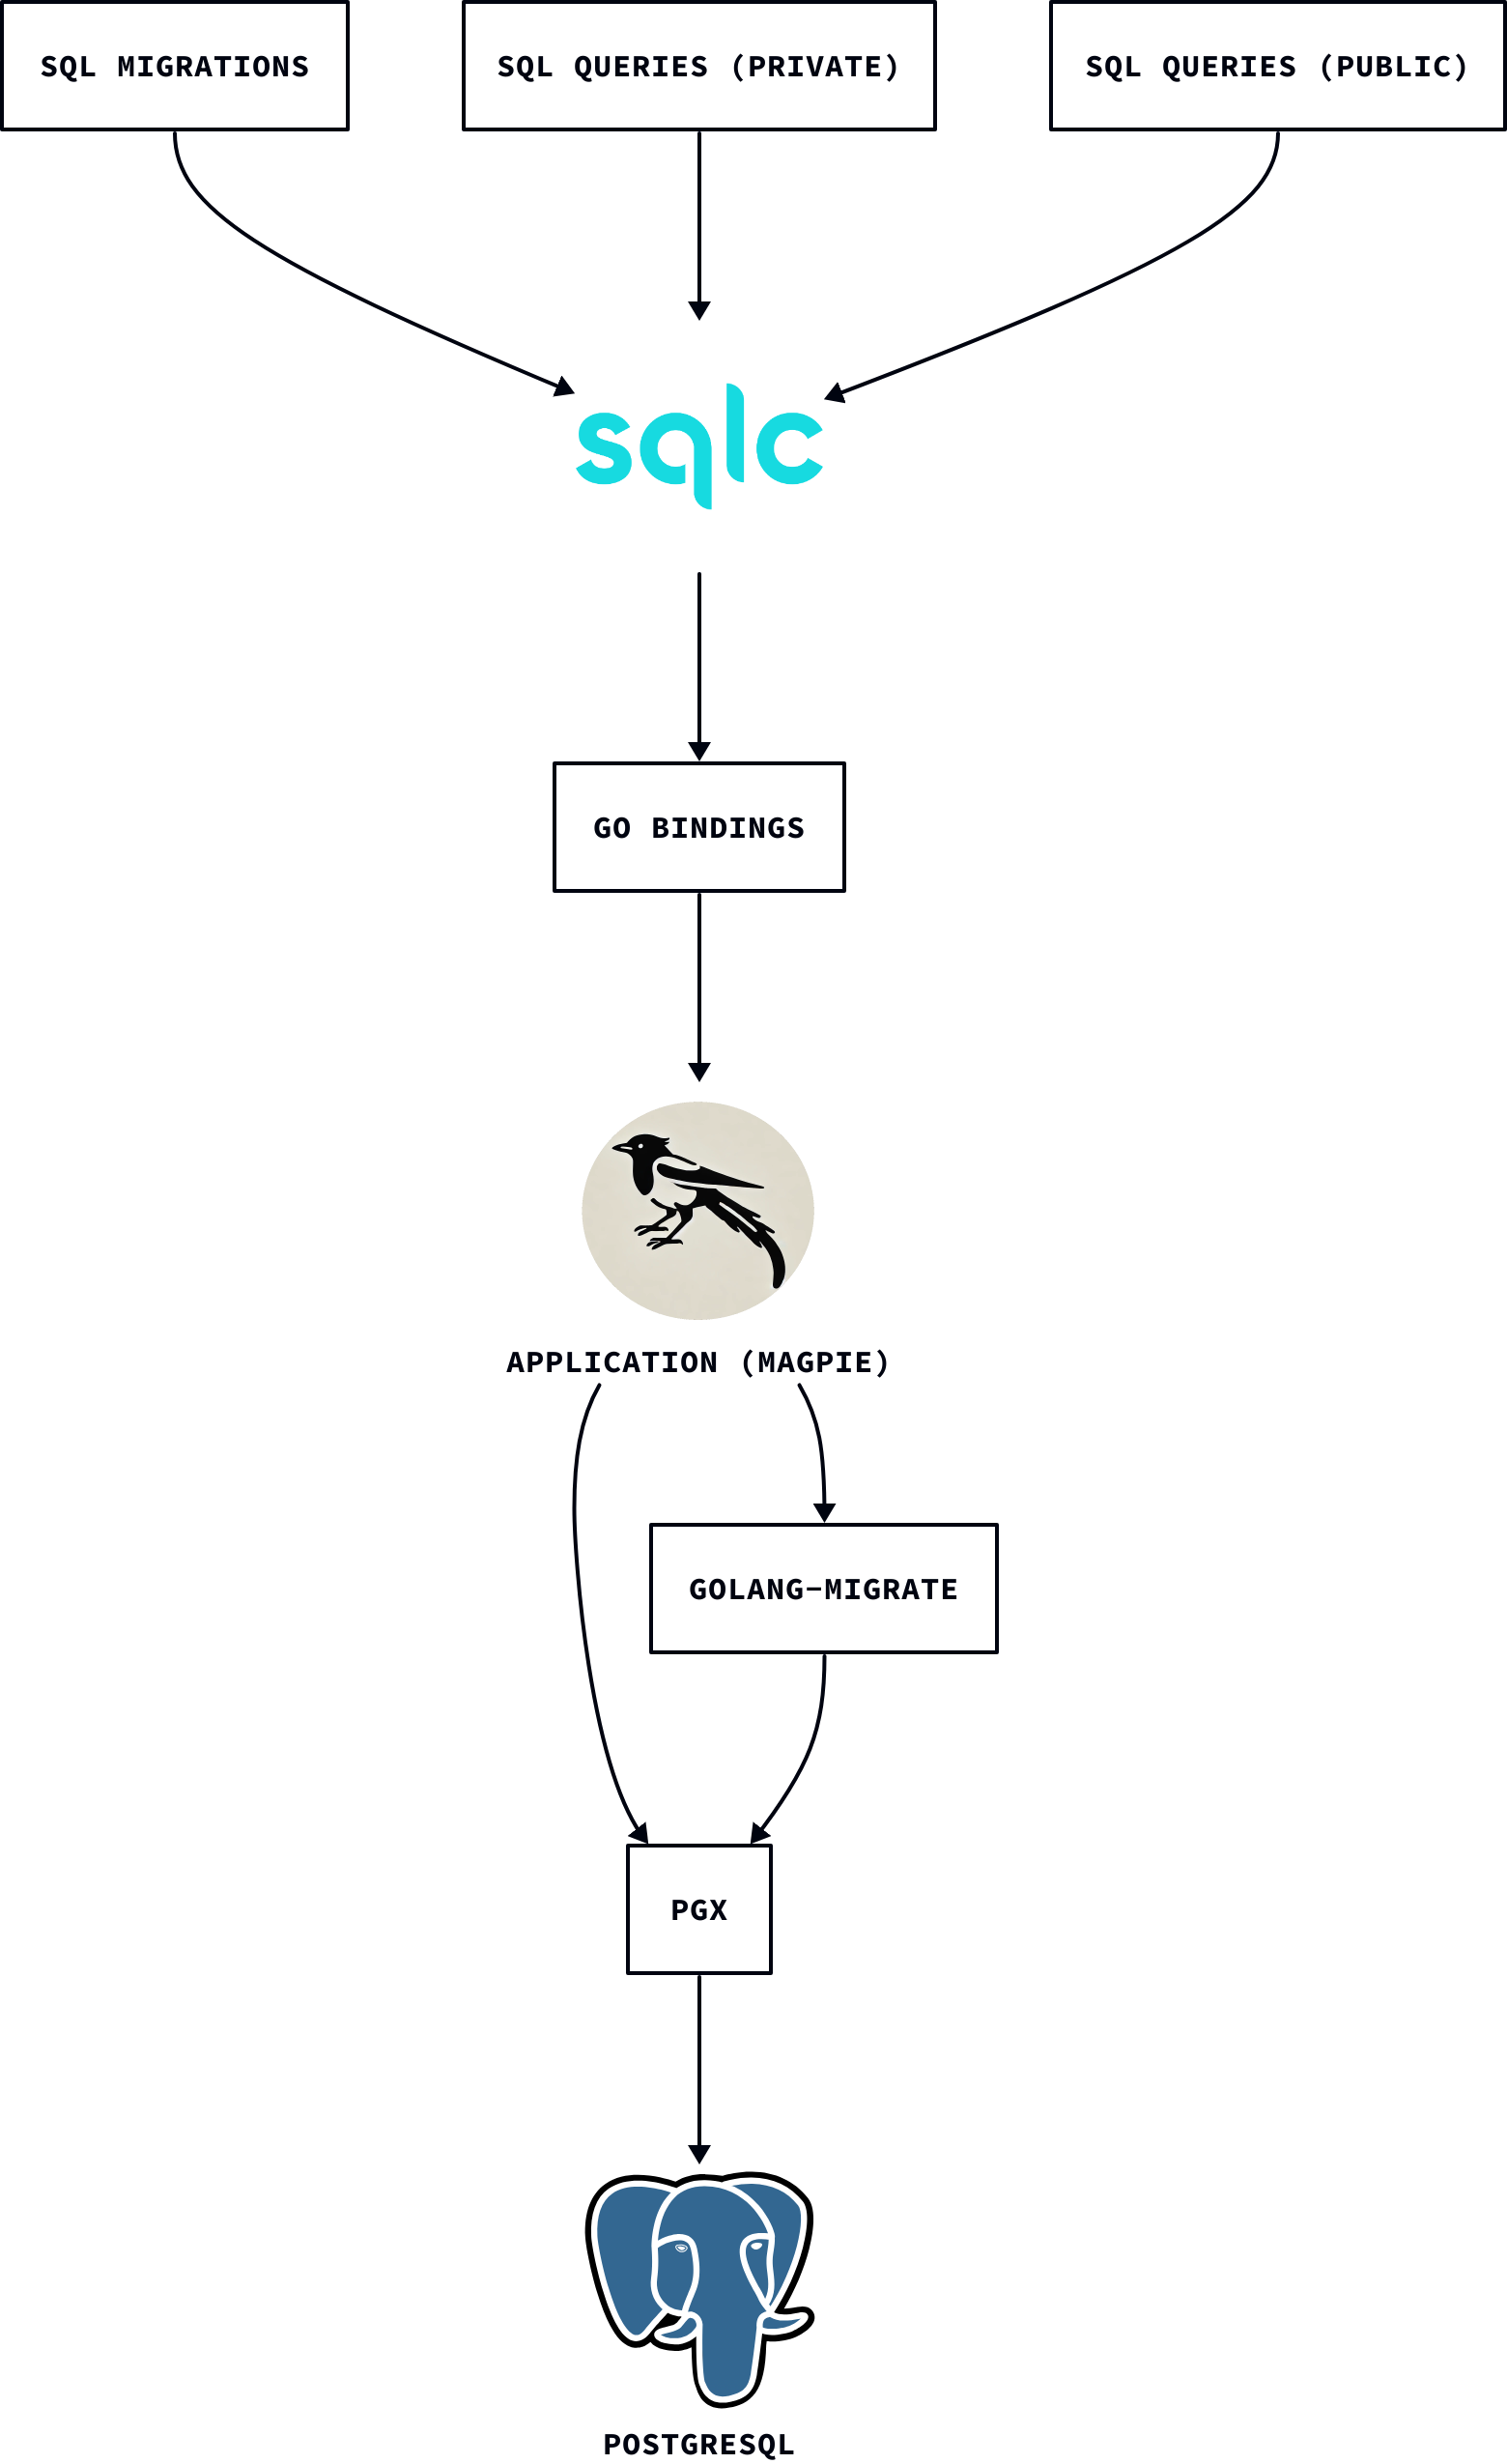
\includegraphics[width=0.8\textwidth]{../d2-diagrams/database_workflow.png}
  \caption{Database Workflow Diagram}
  \label{fig:database_workflow_diagram}
\end{figure}

\paragraph{bcrypt}


\subsubsection{Backend Development}
As discussed in \ref{systemarchitecture} \nameref{systemarchitecture}, the
backend is comprised of two standalone REST-API servers. Right after the
decision to split the backend was taken, a first implementation using two
separate codebases was created. This approach was functional, meaning it was
able to produce two distinct backends with different feature sets.

But it soon became obvious that this approach was not sustainable. While simply
splitting the backend into two codebases was a quick and easy solution, it would
almost certainly lead to significantly increased development times in the
future. The two backends have a fair amount of identical functionality and
differ just in the route handlers and the database queries. Leaving the
codebases separate would result in many changes being made twice -- once in the
private backend and once in the public backend.

After careful consideration and discussions with the team, the decision was made
to revert the change that split the backend. The desired result of two distinct
backends would have to be achieved in a different way.

To accomplish this, a feature of the Go programming language called
\textit{build-tags} was utilised. Usage examples of this feature showcase it by
creating multiple binaries that have different feature sets, for instance
multiple different payment tiers for a single software. This was a great
solution for this problem. It allowed for certain files to be excluded during
compilation based on if they were needed for private or public functionality.
While the development of such a program split by build-tags is more challenging
than developing a single binary, it is much more streamlined than keeping
functionality identical between two separate projects.

\subsubsection{Middlewares}
\paragraph{Authentication}
\paragraph{Authorisation}
\subsubsection{Data Validation}
\subsubsection{Error Handling}
\subsubsection{Testing}